%\begin{enumerate}[label=\arabic*.,ref=\theenumi]
\begin{enumerate}[label=\thesection.\arabic*.,ref=\thesection.\theenumi]
\numberwithin{equation}{enumi}
%2.1.1
\item Consider the Magnitude Bode Plot and Phase Bode Plot \ref{fig:ee18btech11014_Bode} of Open-Loop Transfer Function of an Amplifier. Estimate the Open-Loop Transfer Function. (Assume $'A'$ as $'G'$ and $'\beta'$ as $'H'$)
\begin{figure}[ht!]
	\begin{center}
		\includegraphics[width=\columnwidth]{./figs/ee18btech11014/ee18btech11014_figa.eps}
	\end{center}
	\caption{Magnitude and Phase Bode Plot}
	\label{fig:ee18btech11014_Bode}
\end{figure}
\\
\solution Let $G(f)$ be the Open-Loop Transfer Function,
\begin{align}
G(f) = 
\begin{cases} 
      100 & 0 < f < 10^{5} \\
      200-20\log(f) & 10^{5} < f < 10^{6} \\
      320-40\log(f) & 10^{6} < f < 10^{7} \\
      460-60\log(f) & 10^{7} < f  \\
\end{cases}
\end{align}

\begin{align}
\nabla G(f) &= \dfrac{d(G(f))}{d(\log(f))} =
\begin{cases} 
        0 & 0 < f < 10^{5} \\
      -20 & 10^{5} < f < 10^{6} \\
      -40 & 10^{6} < f < 10^{7} \\
      -60 & 10^{7} < f  \\ 
\end{cases}
\end{align}

As we know that, \textbf{When a pole is encountered the slope always decreases by 20 dB/decade} and \textbf{When a zero is encountered the slope always increases by 20 dB/decade}. So, by observing Fig. \ref{fig:ee18btech11014_Bode} it can be concluded that we are having Poles at $f=10^{5} Hz, 10^{6} Hz, 10^{7} Hz$ and No Zeros.\\

So, the Open-Loop Transfer Function $G(f)$ is
\begin{align}
\label{eq:ee18btech11014_G}
	G(f) = \dfrac{10^{5}}{\left(1+j\frac{f}{10^{5}}\right)\left(1+j\frac{f}{10^{6}}\right)\left(1+j\frac{f}{10^{7}}\right)}
\end{align}\\
%-------------------------------------------------------------------------------------------------%
%2.1.2
\item Calculate the Phase of Open-Loop Transfer Function.\\
\solution
%
\begin{multline}
\label{eq:ee18btech11014_G_ang}
\phi\brak{f} =
\\
-\sbrak{\tan ^{-1}\brak{\frac{f}{10^{5}}}+\tan ^{-1}\brak{\frac{f}{10^{6}}}+\tan ^{-1}\brak{\frac{f}{10^{7}}}}
\end{multline}
%-------------------------------------------------------------------------------------------------%
%2.1.3
\item Find the PM from  Fig. 	\ref{fig:ee18btech11014_Bode}, given that he feedback gain $H(f)$ is constant and given by 
\begin{align}
20 \log \brak{\frac{1}{H(f) }} &= 85 dB
\\
\text{or, } H(f) &= 5.623 \times 10^{-5}.
\end{align}
\\
\solution From the figure, 
\begin{align}
\label{eq:ee18btech11014_G_f1}
20 \log \abs{G(f_1)} &= 85 dB
\\
\implies 20 \log \abs{G(f_1)} & = 20 \log \brak{\frac{1}{H(f_1) }}
\\
\text{or, } \abs{G(f_1)H(f_1)} &= 1
\end{align}
and 
\begin{align}
\label{eq:ee18btech11014_f1}
f_1 = 0.493 MHz, 
\end{align}
from \eqref{eq:ee18btech11014_G_f1} and \eqref{eq:ee18btech11014_G}.
Also,
%
\begin{align}
\because \phase{H(f)} &= 0, \forall f
\\
\phase{G(f_1)H(f_1)} &= \phase{G(f_1)} = -108 \degree
\\
\implies PM &= 180 \degree - 108 \degree = 72 \degree
\end{align}
using \eqref{eq:ee18btech11014_f1} in \eqref{eq:ee18btech11014_G_ang}.

%-------------------------------------------------------------------------------------------------%
\item Find the GM.
\\
\solution The crossover frequency $f_{\pi}$ is defined as 
\begin{align}
\phase{G\brak{f_{\pi}}H\brak{f_{\pi}}} &= 180 \degree
\\
\implies \phase{G\brak{f_{\pi}}} &= 180 \degree
\\
\implies f_{\pi} &= 3.34 MHz
\end{align}
by solving \eqref{eq:ee18btech11014_G_ang}.
From Fig. \ref{fig:ee18btech11014_Bode}, 
\begin{align}
\label{eq:ee18btech11014_G_f1}
20 \log \abs{G(f_\pi)} &= 60 dB
\\
\implies 20 \log \abs{G(f_\pi)} &-  20 \log \brak{\frac{1}{H(f_\pi) }}   
\nonumber \\
&= \brak{60 -85} dB
\\
\implies GM &= \abs{20 \log \abs{G(f_\pi)H(f_\pi) }} 
\nonumber \\
&= 25 dB
\end{align}
%

%------------------------------------------%
%2.1.8
\item Break the Transfer Function $G(f)$ into Simple Blocks and Create a Block Diagram for $G(f)$.\\
\solution\\
\begin{figure}[ht!]
	\begin{center}
		\resizebox{\columnwidth}{!}{\tikzstyle{block} = [draw, rectangle, 
    minimum height=1.5em, minimum width=3em]
\tikzstyle{sum} = [draw, circle, node distance=1cm]
\tikzstyle{input} = [coordinate]
\tikzstyle{output} = [coordinate]
\tikzstyle{pinstyle} = [pin edge={to-,thin,black}]

% The block diagram code is probably more verbose than necessary
\begin{tikzpicture}[auto, node distance=2.5cm,>=latex']
    % We start by placing the blocks
    \node [input, name=input] {};
    \node [block, right of=input] (g) {$10^{5}$};
    \node [block, right of=g] (p1) {$\frac{1}{1+\frac{s}{2\pi \times 10^{7}}}$};
    \node [block, right of=p1] (p2) {$\frac{1}{1+\frac{s}{2\pi \times 10^{6}}}$};
    \node [block, right of=p2] (p3) {$\frac{1}{1+\frac{s}{2\pi \times 10^{5}}}$};
    \node [output, right of=p3] (output) {};

    % Once the nodes are placed, connecting them is easy. 
    \draw [draw,->] (input) -- node {$v_{s}$} (g);
    \draw [->] (g) -- node {$v_{a}$} (p1);
    \draw [->] (p1) -- node {$v_{b}$} (p2);
    \draw [->] (p2) -- node {$v_{b}$} (p3);
    \draw [->] (p3) -- node {$v_{o}$} (output);
    
\end{tikzpicture}
}
	\end{center}
	\caption{}
	\label{fig:ee18btech11014_RC Circuit}
\end{figure}

%-------------------------------------------------------------------------------------------------%
%2.1.9
\item Find the Gain of RC-Circuit in Fig. \ref{fig:ee18btech11014_RC Circuit} and identify the pole location.
\begin{figure}[ht!]
	\begin{center}
		\resizebox{\columnwidth/2}{!}{\begin{circuitikz}[american]
\tikzset{quad/.style={draw, minimum height=2.4cm, minimum width=4cm}}
\node[quad] (A) at (0,0) {$H$};
\draw ($(A.north west)!.175!(A.west)$) to[short,-o] ++(-2,0) -- (-5,1)
      ($(A.south west)!.175!(A.west)$) to[short,-o] ++(-2,0) -- (-5,-1)
      ($(A.north east)!.175!(A.east)$) to[short,-o] ++(1,0)
      ($(A.south east)!.175!(A.east)$) to[short,-o] ++(1,0);

\draw (-5,-1) to[short, i=$I_{f}$] (-5,1);
\draw (-5,-1) to[closing switch, o-o] (-5,-2) node[ground](GND){};

\draw (3,-1) -- (5,-1) to[isource, l= $I_{o}$] (5,1) -- (3,1);

\end{circuitikz}
}
	\end{center}
	\caption{}
	\label{fig:ee18btech11014_RC Circuit}
\end{figure}

\solution
\begin{align}
v_o &= v_i \frac{\frac{1}{sc}}{R + \frac{1}{sC}}
\\
\implies \frac{v_o}{v_i}&= \frac{1}{1+sCR}
%I = \frac{v_{input}}{R + \frac{1}{Cs}}\\
%v_{output} = I \times \frac{1}{Cs}\\
%v_{output} = \frac{v_{input} \times \frac{1}{Cs}}{R + \frac{1}{Cs}}\\
%\frac{v_{output}}{v_{input}} = \frac{1}{RCs + 1}\\
%s = j2\pi f\\
%Gain = \frac{v_{output}}{v_{input}} = \frac{1}{j2\pi RCf + 1}
\end{align}
%
Thus, there is a pole at
%
\begin{align}
s = -\frac{1}{RC}
\end{align}
%

%So, there is a Pole at frequency $f = \frac{1}{2\pi RC}$ for the Transfer Function of Gain.\\
%-------------------------------------------------------------------------------------------------%
%2.1.10
\item Find the Gain of Operational Amplifier. The circuit diagram of Equivalent Circuit is \ref{fig:ee18btech11014_OpAmp Circuit}.
\begin{figure}[ht!]
	\begin{center}
		\resizebox{\columnwidth}{!}{\begin{circuitikz}[american]
\ctikzset{tripoles/mos style/arrows}

\draw (0,0) node[ground](GND){} to[vsourcesin, l= $v_{c}$] (0,4) to[R=$R_{s}$] (2,4) to[short, -o] (2.25,4) node[label={below:$+$}]{};
\draw (2.25,2) to[R=$R_{1}$, v=$v_{f}$] (2.25,0) node[ground](GND){};
\draw (2.25,2) to[short, -o] (2.25,2.25) node[label={above:$-$}]{};
\draw (2.25,2.65) node[label={$v_{i}$}]{};
\draw (2.25,2.25) -- (3,2.25) to[R=$R_{2}$] (5,2.25) -- (5,4) -- (6,4) to[vsourcesin, l=$Gv_{i}$] (6,0) node[ground](GND){};
\draw (6,4) -- (8.5,4) to[R=$R_{L}$] (8.5,0) node[ground](GND){};
\draw (8.5,4) to[short,-o] (9,4) node[label={above:$v_{o}$}]{};
\end{circuitikz}
}
	\end{center}
	\caption{}
	\label{fig:ee18btech11014_OpAmp Circuit}
\end{figure}

\solution\\
Applying KVL and KCL,
\begin{align}
v_{o} = Gv_{i}
\end{align}

As no current flows through $R_{s}$,
\begin{align}
v_{i} = v_{c} - v_{f}\\
v_{f} = \frac{R_{1}}{R_{1}+R_{2}}v_{o}\\
v_{i} = \frac{v_{o}}{G}\\
\frac{v_{o}}{G} = v_{c} - \frac{R_{1}}{R_{1}+R_{2}}v_{o}\\
\frac{v_{o}}{v_{c}} = \frac{G}{1+G\frac{R_{1}}{R_{1}+R_{2}}}
\end{align}

So, Gain of the Circuit is $\frac{G}{1+G\frac{R_{1}}{R_{1}+R_{2}}}$
%-------------------------------------------------------------------------------------------------%
%2.1.11
\item Design a Circuit Model that follows the Transfer Function $G(f)$\\
\solution\\
Our Design for Modelling the Transfer Function is based on Poles of RC-Circuit and Gain of Operational Amplifier.\\

So, the Circuit Diagram is,
\begin{figure}[ht!]
	\begin{center}
		\resizebox{\columnwidth/1}{!}{\begin{circuitikz}[american]

\draw (2,2)  node[op amp] (OA) {};
\draw (OA.up) -- ++(0, 0.3) node[vcc]{$+10V$};
\draw (OA.down) -- ++(0,-0.3) node[vee]{$-10V$};
\draw (OA.+) -- (0,1.5) to[vsourcesin, l= $v_{s}$] (0,0) node[ground](GND){};
\draw (OA.-) -- (0,2.5) node[ground, rotate=270](GND){};
\draw (OA.out) -- (3,2) node[label={above:$v_{a}$}]{};
\draw (3,2) to[R=$R_{1}$] (5.5,2) node[label={above:$v_{b}$}]{} to[C,l_=$C_{1}$] (5.5,0) node[ground](GND){};
\draw (5.5,2) to[R=$R_{2}$] (8,2) node[label={above:$v_{c}$}]{} to[C,l_=$C_{2}$] (8,0) node[ground](GND){};
\draw (8,2) to[R=$R_{3}$] (10.5,2) to[C,l_=$C_{3}$] (10.5,0) node[ground](GND){};
\draw (10.5,2) -- (11.5,2) node[label={above:$v_{o}$}]{};

\end{circuitikz}
}
	\end{center}
	\caption{}
	\label{fig:ee18btech11014_Open-Loop Circuit}
\end{figure}
 
Assuming, Open-Loop Gain of Operational Amplifier is $10^{5}$ and also assuming Operational Amplifier doesnt have any Poles.\\
Equivalent Circuit of the circuit is
\begin{figure}[ht!]
	\begin{center}
		\resizebox{\columnwidth/1}{!}{\begin{circuitikz}[american]
\ctikzset{tripoles/mos style/arrows}
\draw (0,0) node[ground](GND){} -- (0,2) to[short, -o] (0.5,2) -- (0.5,2) to[R=$R_{F}$,i=$I_{F}$] (3,2);
\draw (1,2) node[label={below:Port-1}]{};
\draw (3,2) to[R=$R_{M}$] (3,0) node[ground](GND){};
\draw (3,2) to[short, -o] (4,2) -- (5.5,2);
\draw (4,2) node[label={above:Port-2}]{};
\draw (5.5,0) node[ground](GND){} to[isource, l= $I_{o}$] (5.5,2);
\end{circuitikz}
}
	\end{center}
	\caption{}
	\label{fig:ee18btech11014_Equivalent Open-Loop Circuit}
\end{figure}

The cascade of RC Circuits are used to introduce poles in the circuit and Op-Amp are used to achieve the Gain required.\\

At the Operational Amplifier,
\begin{align}
v_{i} = v_{s}\\
v_{a} = 10^5 v_{i}\\
v_{a} = 10^5 v_{s}
\end{align}

At the first RC-Circuit,
\begin{align}
2\pi RC = 10^{-7}\\
v_{b} = \frac{v_{a}}{1 + j\frac{f}{10^{7}}}\\
v_{b} = \frac{10^5 v_{i}}{1 + j\frac{f}{10^{7}}}
\end{align}

At the second RC-Circuit,
\begin{align}
2\pi RC = 10^{-6}\\
v_{c} = \frac{v_{b}}{1 + j\frac{f}{10^{6}}}\\
v_{c} = \frac{10^5 v_{i}}{(1 + j\frac{f}{10^{6}})(1 + j\frac{f}{10^{7}})}
\end{align}

At the third RC-Circuit,
\begin{align}
2\pi RC = 10^{-5}\\
v_{o} = \frac{v_{c}}{1 + j\frac{f}{10^{5}}}
\end{align}
\begin{align}
v_{o} = \frac{10^5 v_{i}}{(1 + j\frac{f}{10^{5}})(1 + j\frac{f}{10^{6}})(1 + j\frac{f}{10^{7}})}
\end{align}

The RC Circuits introduces poles at $f=10^{7} Hz, 10^{6} Hz, 10^{5} Hz$ respectively from left to right and Op-Amp introduced a Gain = $10^5$. So, the value of $v_{o}$ is

\begin{align}
v_{o} = \dfrac{10^5 v_{i}}{\left(1+j\frac{f}{10^{5}}\right)\left(1+j\frac{f}{10^{6}}\right)\left(1+j\frac{f}{10^{7}}\right)}
\end{align}

So, Open-Loop Gain is
\begin{align}
G = \dfrac{10^5}{\left(1+j\frac{f}{10^{5}}\right)\left(1+j\frac{f}{10^{6}}\right)\left(1+j\frac{f}{10^{7}}\right)}
\end{align}
%-------------------------------------------------------------------------------------------------%
%2.1.12
\item Design a Circuit Model that follows the Feedback Transfer Function $H(f)$\\
\solution\\
On Bode Plot is $H$ is independent of frequency. So, $H$  should not involve any Reactive Elements. So, $H$ is a combination of Resistors or a Voltage Divider.
\begin{figure}[ht!]
	\begin{center}
		\resizebox{\columnwidth/2}{!}{\begin{circuitikz}[american]
\ctikzset{tripoles/mos style/arrows}
\draw (1,2) to[short, -o] (0,2) node[label={below:$v_{o}$}]{};
\draw (1,2) to[R=$R_{M}$] (2,2) -- (3,2) to[R=$R_{F}$] (3,0) node[ground](GND){};
\draw (3,2) to[short, -o] (4,2) node[label={below:$v_{f}$}]{};
\end{circuitikz}
}
	\end{center}
	\caption{}
	\label{fig:ee18btech11014_Feedback Circuit}
\end{figure}

\begin{align}
v_{f} = \frac{10}{10 + 1.778\times 10^{5}} \times v_{o}\\
v_{f} \approx 5.623\times 10^{-5} v_{o}\\
\frac{v_{f}}{v_{o}} \approx 5.623\times 10^{-5}\\
H(f) = 5.623\times 10^{-5}
\end{align}
%-------------------------------------------------------------------------------------------------%

\item Draw the Magnitude and Phase Bode Plots of $G(f)$\\
\solution
Magnitude Plot is \ref{fig:Magnitude Plot}
\begin{figure}[ht!]
	\begin{center}
		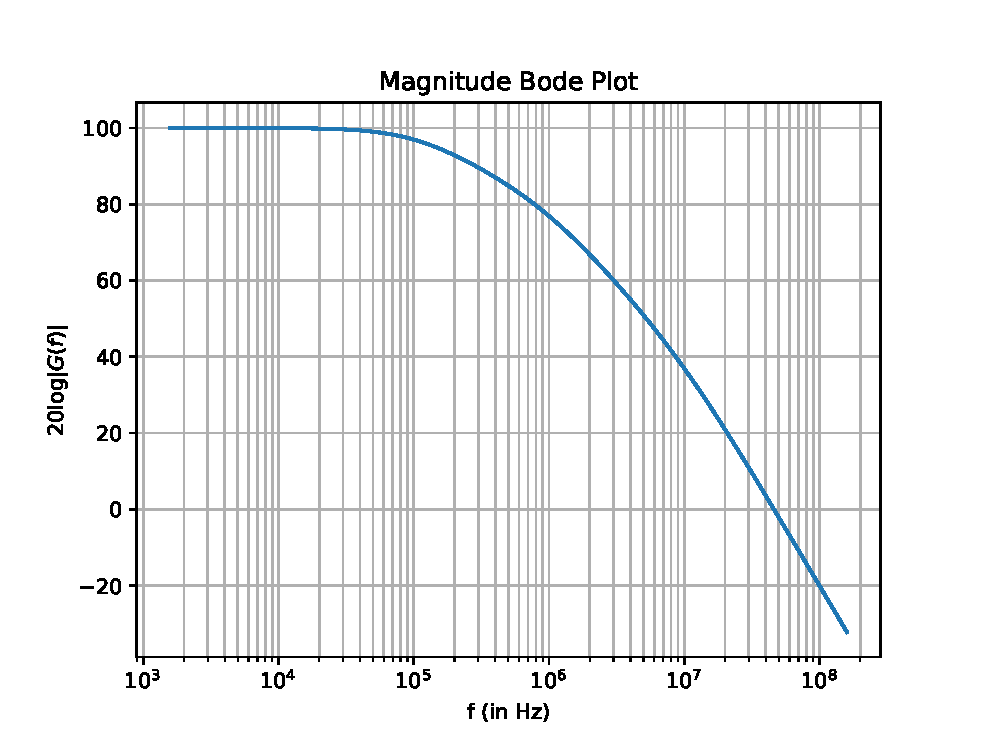
\includegraphics[width=\columnwidth]{./figs/ee18btech11014/Magnitude_Plot.eps}
	\end{center}
	\caption{Magnitude Bode Plot}
	\label{fig:Magnitude Plot}
\end{figure}

Phase Plot is \ref{fig:Phase Plot}
\begin{figure}[ht!]
	\begin{center}
		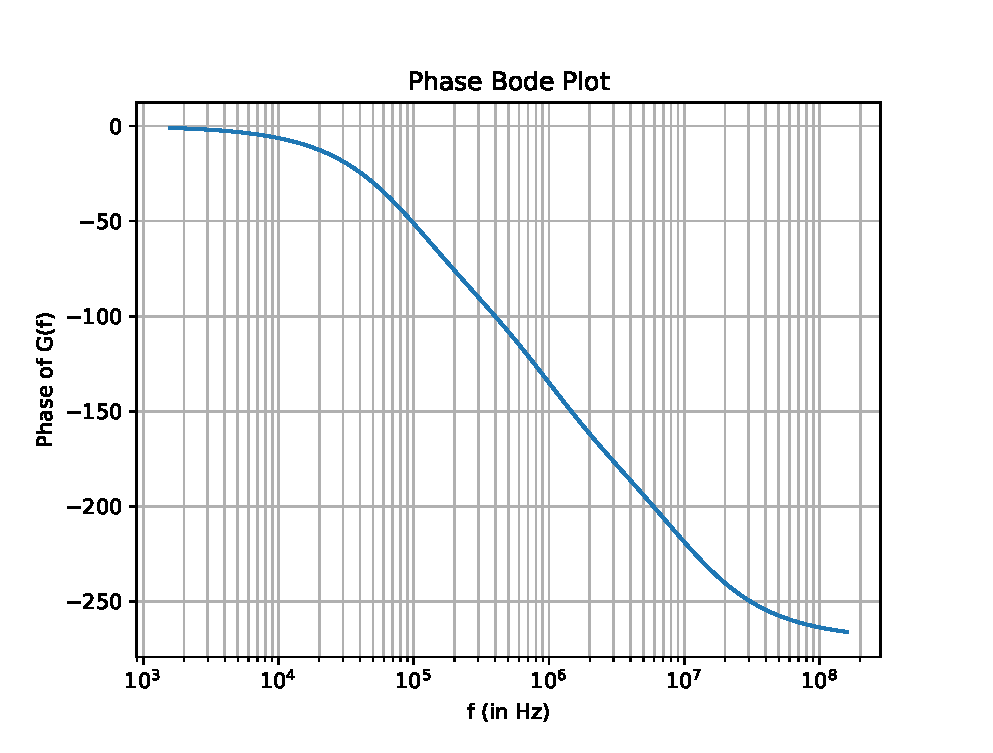
\includegraphics[width=\columnwidth]{./figs/ee18btech11014/Phase_Plot.eps}
	\end{center}
	\caption{Phase Bode Plot}
	\label{fig:Phase Plot}
\end{figure}

Python Code for Magnitude and Phase Bode Plots is at
\begin{lstlisting}
codes/ee18btech11014/Bode_Plot.py
\end{lstlisting}

%-------------------------------------------------------------------------------------------------%
%2.1.13
\item  Design a Closed-Loop Transfer Function by combining both the Open-Loop and Feedback Circuits. Also draw its Equivalent Circuit\\
\solution\\
The Closed-Loop Circuit is
\begin{figure}[ht!]
	\begin{center}
		\resizebox{\columnwidth}{!}{\begin{circuitikz}[american]

\draw (2,2)  node[op amp] (OA) {};
\draw (OA.up) -- ++(0, 0.3) node[vcc]{$+10V$};
\draw (OA.down) -- ++(0,-0.3) node[vee]{$-10V$};
\draw (OA.+) -- (0,1.5) to[vsourcesin, l= $v_{s}$] (0,0) node[ground](GND){};
\draw (OA.-) -- (0,2.5) to[R=$10\ohm$] (-2,2.5) node[ground, rotate=270](GND){};
\draw (OA.out) -- (3,2) node[label={below:$v_{a}$}]{};
\draw (3,2) to[R=$10^{2}\ohm$] (5.5,2) node[label={above:$v_{b}$}]{} to[C,l_=$\frac{10^{-9}}{2\pi}F$] (5.5,0) node[ground](GND){};
\draw (5.5,2) to[R=$10^{3}\ohm$] (8,2) node[label={above:$v_{c}$}]{} to[C,l_=$\frac{10^{-9}}{2\pi}F$] (8,0) node[ground](GND){};
\draw (8,2) to[R=$10^{4}\ohm$] (10.5,2) to[C,l_=$\frac{10^{-9}}{2\pi}F$] (10.5,0) node[ground](GND){};
\draw (10.5,2) -- (11.5,2) node[label={above:$v_{o}$}]{};
\draw (10.5,2) -- (10.5,4) to[R=$1.778\times 10^{5}\ohm$] (0,4) -- (0,2.5);

\end{circuitikz}
}
	\end{center}
	\caption{}
	\label{fig:ee18btech11014_Closed-Loop Circuit}
\end{figure}

The Equivalent Circuit of Closed-Loop Circuit is
\begin{figure}[ht!]
	\begin{center}
		\resizebox{\columnwidth}{!}{\begin{circuitikz}[american]-1
\draw (-3,0) node[ground](GND){} to[vsourcesin, l= $v_{s}$] (-3,2) to[short,-o] (0.25,2) node[label={below:$+$}]{};
\draw (0,0.1) to[R=$10\ohm$,v=$v_{f}$] (-2,0.1) node[ground](GND){}; 
\draw (0,0.1) -- (1,0.1) -- (1,4) to[R=$1.778\times 10^{5}\ohm$] (10.5,4) -- (10.5,2);


\draw (0.25,0.1) to[short,-o] (0.25,0.1) node[label={above:$-$}]{};
\draw (0.25,0.625) node[label={$v_{i}$}] {};


\draw (3,2) node[label={above:$v_{a}$}]{};
\draw (3,0) node[ground](GND){} to[vsourcesin, l= $10^5 v_{i}$] (3,2);
\draw (3,2) to[R=$10^{2}\ohm$] (5.5,2) node[label={above:$v_{b}$}]{} to[C,l_=$\frac{10^{-9}}{2\pi}F$] (5.5,0) node[ground](GND){};
\draw (5.5,2) to[R=$10^{3}\ohm$] (8,2) node[label={above:$v_{c}$}]{} to[C,l_=$\frac{10^{-9}}{2\pi}F$] (8,0) node[ground](GND){};
\draw (8,2) to[R=$10^{4}\ohm$] (10.5,2) to[C,l_=$\frac{10^{-9}}{2\pi}F$] (10.5,0) node[ground](GND){};
\draw (10.5,2) -- (11.5,2) node[label={above:$v_{o}$}]{};

\end{circuitikz}
}
	\end{center},
	\caption{}
	\label{fig:ee18btech11014_Closed-Loop Equivalent Circuit}
\end{figure}

From the Equivalent Circuit Diagram,
\begin{align}
G = \frac{v_{o}}{v_{i}} = \dfrac{10^5}{\left(1+j\frac{f}{10^{5}}\right)\left(1+j\frac{f}{10^{6}}\right)\left(1+j\frac{f}{10^{7}}\right)}\\
H = \frac{v_{f}}{v_{o}} = 5.623 \times 10^{-5}
\end{align}

The Closed-Loop Gain,
\begin{align}
v_{i} = v_{s} - v_{f}\\
\frac{v_{o}}{G} = v_{s} - Hv_{o}\\
\frac{v_{o}}{v_{s}} = \frac{G}{1+GH}
\end{align}

So, the Closed-Loop Gain,
\begin{align}
T = \frac{v_{o}}{v_{s}} = \dfrac{10^5}{5.623 + \left(1+j\frac{f}{10^{5}}\right)\left(1+j\frac{f}{10^{6}}\right)\left(1+j\frac{f}{10^{7}}\right)}
\end{align}

\end{enumerate}
